\documentclass[a4paper]{article}
\usepackage[letterpaper, margin=1in]{geometry} % page format
\usepackage{listings} % this package is for including code
\usepackage{graphicx} % this package is for including figures
\usepackage{amsmath}  % this package is for math and matrices
\usepackage{amsfonts} % this package is for math fonts
\usepackage{hyperref} % for urls

\title{Midterm Questions!}
\author{Morgan Baker}
\date{10/13/16}

\begin{document}
\lstset{language=Python}

\maketitle

\section{Question 1}
This was the question from the past homework. The question asks us to take a dataset of 7291 points located in a csv file, and asks us to sort them using three different approaches. The first approach uses the pocket algorithm. I figured out the error in the old code. I kept getting instance variables mixed with local variables. However, it works now, and the output for the code can be found at Figure \ref{fig:Figure1}. The Eout for this method came to be .012069674941708956 after 916 iterations. Linear Regression calculated it's Eout at .01522424907420107, which is worse than the pocket algorithm. The worst is with the thrid algorithm, or the best of both worlds algorithm from before. It isn't necessarily the best of both worlds though, because the pocket algorithm got to the same Eout, but took about 350 more iterations, as shown in Figure \ref{fig:Figure2}. This means that in this case, the pocket algorithm by itself seems like the best bet. 
\begin{figure}
  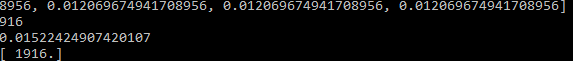
\includegraphics[width=\linewidth]{figure1.png}
  \caption{The Eout of the Pocket Algorithm and Linear Regression separately.}
  \label{fig:Figure1}
\end{figure}
\begin{figure}
  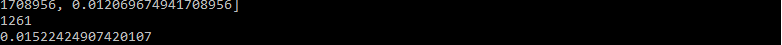
\includegraphics[width=\linewidth]{figure2.png}
  \caption{The Eout and iterations of the Pocket Algorithm that startted with the weights from Linear Regression.}
  \label{fig:Figure2}
\end{figure}
\section{Question 2}
The second question is something that I had wanted to do for homework 2, but instead threw it in a graphing calculator. The quesiton asks us to make the equation from problem 2.12 to run iteratively. This is done by creating the Equation.py class. This class takes the equation\\
$N\geq\frac{8}{\varepsilon^2}ln(\frac{4((2N)^{10}+1)}{\delta})$\\
 and applies it to the problem. It then loops until N is equal to itself with the accuracy of about 15 decimals. It then takes the data and plots it, as shown in Figure \ref{fig:Figure3}. This was a fun problem to work on. 
 \begin{figure}
  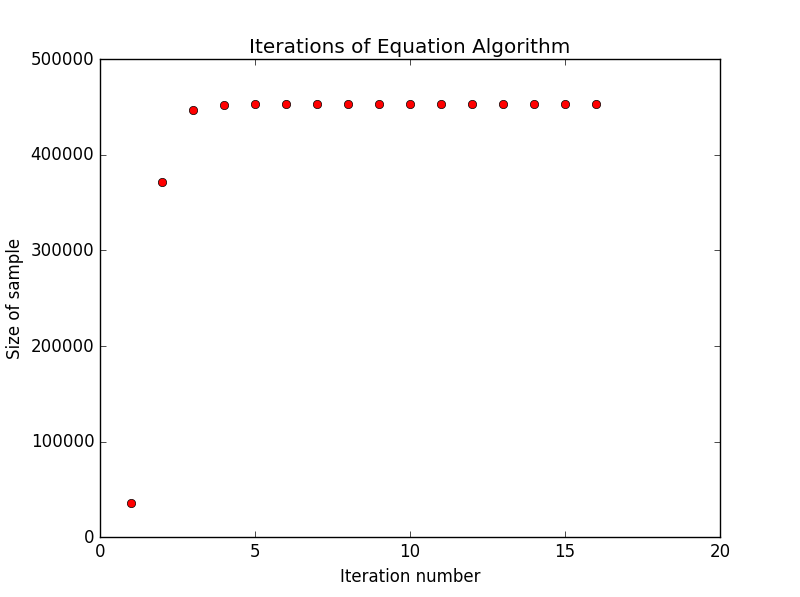
\includegraphics[width=\linewidth]{plot.png}
  \caption{The plot of samples to the number of iteraitons.}
  \label{fig:Figure3}
  
\section{Question 3}
I wasn't really sure what to do for this, since I'm not necessarily the best artist. I can tell you that when we were first talking about Perceptrons, I saw them as another type of Transformer. ''Oh no, the Perceptrons are coming'', ''Don't worry class, I can help with this''  runs preceptron learning algorithm... Yeah this is weird.
  \end{figure}
\end{document}